\documentclass{article}
\usepackage[utf8]{inputenc}
\usepackage{caratula}
\usepackage{graphicx}
\usepackage{verbatim}
% \title{}
% \author{  \\ Ezequiel Reiner \\ Natalia Pesaresi}
% \date{July 2018}

\begin{document}

\thispagestyle{empty}
\materia{Teoria de Lenguajes}
\submateria{Primer Cuatrimestre de 2018}
\titulo{Conversor de JSON a YAML}
%\subtitulo{Procesamiento de imágenes}

\integrante{Regnier, Ezequiel}{836/13}{eze\_regnier@hotmail.com}
\integrante{Zamboni, Gianfranco}{219/13}{gianfranco375@gmail.com}
\integrante{Pesaresi, Natalia}{636/14}{natalia.pesaresi@gmail.com}

\maketitle

\newpage

\tableofcontents
\newpage

\section{Introducción}

En este trabajo, se propone realizar un conversor de código JSON a código YAML. Ambos lenguajes poseen las mismas estructuras, por lo que hay equivalencias sintácticas entre ellos. \\ \\
Por ejemplo en el caso de los arrays: \\

\begin{center}
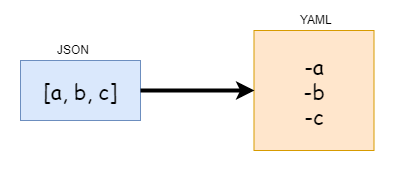
\includegraphics[scale=0.7]{img1.png}
\end{center}

Para realizar esta conversión, se necesita un Lexer que reconozca las cadenas que pertenecen al lenguaje JSON. Y un parser que traduzca sintácticamente la escritura a YAML. \\

\section{Gramática}

La siguiente gramática G, genera el lenguaje aceptado por el lenguaje JSON. \\
G=\{ \{Value, Object, Array, Members, Pair, Elements\}, \{string, number, true, false, null, [, ], \{, \}, : \}, Value, P \} \\ \\
Donde P: \\

\begin{center}
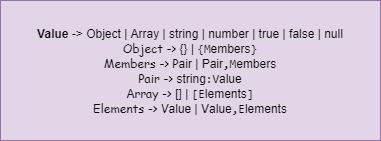
\includegraphics[scale=0.9]{img2.png}
\end{center}

Una carasterística importante que se necesitaconocer, a la hora de hacer el parser, es su tipo. Se quizo analizar si la gramática es LALR(1). Para ello, se utoilizó una herramienta que genera para una grámatica su tabla LALR. [-1-]
\begin{center}
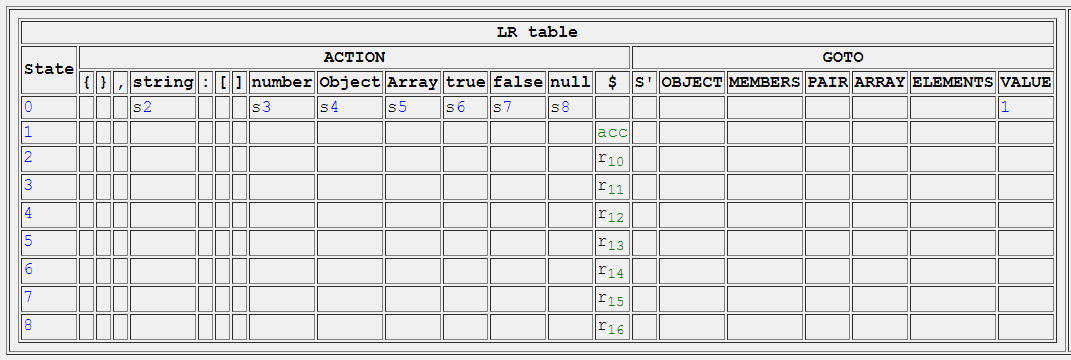
\includegraphics[scale=0.55]{img3.png}
\end{center}
Como la tabla no presenta conflictos, se concluye que la gramática es LALR(1),

\section{Lexer}

Para generar el Lexer, se utilizó la biblioteca de python Lex. \\ \\
La estructura del lexer tiene las siguientes características:
\begin{itemize}
    \item Definición de los tokens que posee la gramática
    \item Definición de las funciones t\_NUMBER y t\_STRING donde se especifica la forma de los números y cadenas de caracteres que acepta la gramática. Por ejemplo: '1.0' será un numero válido, pero '1.0ee' no.
    \item Definición de las funciones t\_error y t\_newline que son necesarias por la biblioteca para mostrar un mensaje de error cuando sea requerido e identificar un salto de línea respectivamente.
\end{itemize}
Por último, se define la instanciación del lexer de la siguiente manera: lexer = lex.lex().

\section{Parser}
Para generar el Parser, se utilizó la biblioteca de python Yacc. Éste toma el árbol de tokens credo por el Lexer.\\ \\
Se crean tantas funciones como no terminales existan. Cada una de ellas acepta un único argumento 'p' que es un arreglo de elementos p asociados a los terminales y no teminales de la producción que tiene como parte derecha, que corresponde a la función. \\
Por elemplo en la función p\_object:
\begin{verbatim}
def p_object(p):
    '''object : LLAVEIZQ LLAVEDER'''
    ...
\end{verbatim}
Aquí p = [p\_0,p\_1,p\_2].
\\ \\
Un dato relevante es que 'p' tiene un sólo atributo 'value' que debe ser 'sintetizado'. \\ \\
Durante la ejecución del parser se genera lo que llamamos 'Parsing Tree', esto es el árbol de objetos 'p' que se genera a partir de las sucesivas llamadas a función. \\
Por ejemplo, al parsear: [a, b, c]. El 'Parsing Tree' será el árbol: p\_Value $\rightarrow$ p\_Object $\rightarrow$ [ p\_Members ] $\rightarrow$Value , p\_Elements $\rightarrow$ Value , p\_Elements $\rightarrow$ Value 
\\ \\
En este trabajo, por las características del código YAML, era deseable contar con un atributo TABS 'heredado', y un atributo CADENA 'sintetizado'. Por lo expresado anteriormente, esto no era posible, por lo que se debió modificar la estrategia de diseño del parser. \\ \\
Se procedió a crear la Clase TokkenWithAttributes:
\begin{center}
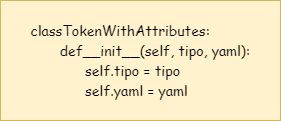
\includegraphics[scale=.8]{img4.png}
\end{center}
Por lo tanto ahora los elementos 'p', son del tipo TokkenWithAttributes.
El atributo Tipo, es un string y el atributo 'Yaml' es una función que toma como parámetro los tabs correspondientes a la posición del objeto actual.
\\ \\
La estructura final del parser es:
\begin{itemize}
    \item Se generó el 'Parsing Tree'. $parsedValue = p[1]$
    \item Se utilizó el atributo 'Yaml' del parsedValue, para imprimir la traducción. \\ %Este atributo es una función que toma por parámetro los tabs correspondientes al elemento actual. De esta manera se puede conseguir una simulación de nuestro requerimiento anterior para calcular los tabs de cada elemento aprovechando el parsing tree generado, sin crear un atributo 'heredado'.
\end{itemize}

\section{Desiciones de diseño}
Para realizar la conversión de código JSON a YAML se precisó utilizar el estilo 'double-quoted', que conciste en explicitar el tipo string de una cadena agregándole comillas, ya que había 2 conflictos: \\
\textbf{Cadenas de un tipo que podían confundirse con otro.} Por ejemplo, si tenemos la cadena -Cadena3 como clave de un objeto, a simple vista pareciera ser un item de un arreglo, cuando no lo es. \\
\textbf{Otro conflicto se presenta cuando tenemos un catacter como '\texttt{\textbackslash n}',} ya que se necesita una representación para el salto de línea. \\
\textbf{Decidimos utilizar el estilo para la representación de todas las direcivas '\texttt{\textbackslash x}',} ya que nos parece adecuado para la traducción.


\section{Pruebas}

Corrimos el parser para los archivos de prueba jasonObjet1.txt y jasonObjet2.txt con código JSON, y sus respectivas traducciones a código YAML fueron res1.txt y res2.txt.

\section{Requerimientos de Software}

\begin{itemize}
    \item Python, Version: 2.6
    \item PLY, Version: 3.5
\end{itemize}

\section{Comando de ejecución}
Para ejecutar el trabajo es necesario escribir por entrada standard un objeto JSON. Por lo que un ejemplo es:
\begin{itemize}
    \item python3 tptleng.py $<$objeto$\_$JSON.txt
\end{itemize}

\section{Referencias}
[-1-] Página: \begin{verbatim}http://jsmachines.sourceforge.net/machines/lalr1.html\end{verbatim}.

\end{document}
